\documentclass[tikz]{standalone}
\usepackage{tikz}
\usepackage{pgfplots}

\begin{document}    
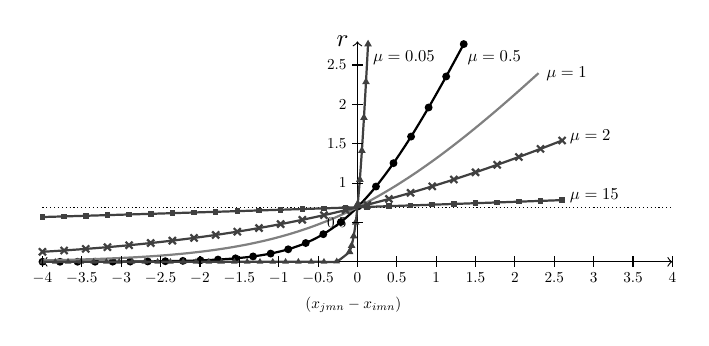
\begin{tikzpicture}
 \usetikzlibrary{positioning}
 \node (center) {};
 
 
 %Coordinates
 \coordinate (RRMcoordinate) at (0.5,1);

 
 %Name

  \node (rejoice) [scale=0.6,above right=1.3cm and 2.5cm of center,black ] {$\mu=2$};
    \node (rejoice) [scale=0.6,above right=2.1cm and 2.2cm of center,black ] {$\mu=1$};
    \node (rejoice) [scale=0.6,above right=2.3cm and 1.2cm of center,black ] {$\mu=0.5$};
    
    \node (rejoice) [scale=0.6,above right=2.3cm and 0cm of center,black ] {$\mu=0.05$};
    \node (rejoice) [scale=0.6,above right=0.55cm and 2.5cm of center,black ] {$\mu=15$};
 %Axis
   \draw[<->] (-4, 0) -- (4, 0) node[scale=0.55,below left= 0.25cm and -.75cm of center] {$(x_{jmn} - x_{imn})$};
  \draw[->] (0,0 ) -- (0, 2.8) node[left,scale=0.9] {$r$};
  
 %Functions mark=*,samples=3,mark options={scale=0.5} 
 
 
      \draw[scale=1, domain=-4:1.35, smooth ,variable=\x, black,thick,mark=*,mark options={scale=0.5} ] plot  ({\x}, {ln(1+exp(\x/0.5))});

   \draw[scale=1, domain=-4:2.3, smooth ,variable=\x, gray,thick] plot  ({\x}, {ln(1+exp(\x))});
   

      \draw[scale=1, domain=-4:2.6, smooth ,variable=\x, darkgray,thick,mark=x,mark options={scale=0.9}] plot  ({\x}, {ln(1+exp(\x/2))});
      
  \draw[scale=1, domain=-4:4, densely dotted ,variable=\x, black] plot  ({\x}, {ln(2)});

      \draw[scale=1, domain=-4:2.6, smooth ,variable=\x, darkgray,thick,mark=square*,mark options={scale=0.3}] plot  ({\x}, {ln(1+exp(\x/15))});

\draw[scale=1, domain=-4:-.1, smooth ,variable=\x, darkgray,thick,mark=triangle,mark options={scale=0.3}] plot  ({\x}, {ln(1+exp(\x/0.05))});

\draw[scale=1, domain=-.1:0.135, smooth ,variable=\x, darkgray,thick,mark=triangle,mark options={scale=0.4},samples=10] plot  ({\x}, {ln(1+exp(\x/0.05))});


 \foreach \x/\xtext in {0,0.5,1,1.5,2,2.5,3,3.5,4}
\draw[shift={(\x,0)}] (0pt,2pt) -- (0pt,-2pt) node[scale=0.55,below] {$\xtext$};

 \foreach \x/\xtext in {0.5,1,1.5,2,2.5,3,3.5,4}
\draw[shift={(-\x,0)}] (0pt,2pt) -- (0pt,-2pt) node[scale=0.55,below] {$-\xtext$};

  \foreach \y/\ytext in {0.5,1,1.5,2,2.5}
  \draw[shift={(0,\y)}] (2pt,0pt) -- (-2pt,0pt) node[scale=0.55,left] {$\ytext$};
  %Labels of functions


 % \draw[->] (RRM) -- (RRMcoordinate);

  
\end{tikzpicture}
\end{document}


